\chapter{Components of a CNN}
% Authors: Joanna Bitton, Divyansh Khanna, Lind Xiao, 2/26/19.

\section{Variety of layers}
% Authors: Joanna Bitton, Divyansh Khanna, Lind Xiao, 2/26/19.
A convolutional neural network may consist of various kinds of layers.
Each layer is responsible for extracting relevant information and creating higher-level interpretations of the input.
In a standard CNN, an input will go through a series of layers such as convolution, non-linearity, pooling, and batch normalization layers.

\subsection{Convolution}
% Authors: Joanna Bitton, Divyansh Khanna, Lind Xiao, 2/26/19.
A convolution layer is the backbone of all convolutional neural networks.
The layer contains a set of learnable filters that will produce an activation map displaying how the input has responded to each filter.
For instance, a filter could attempt to detect a certain kind of edge present in the input, or in higher levels of the network detect a shape.
This is achieved by using small spatial filters that convolve over the height and width of the image, computing the dot product at every position.
The output of each filter will produce a two-dimensional activation map which will be stacked along the depth-dimension to create the output for the layer.

\subsection{Non-linearity}
% Authors: Joanna Bitton, Divyansh Khanna, Lind Xiao, 2/26/19.
Without a non-linearity module present in the network, no matter how many layers are defined, the neural network would behave like a single-layered model. 
This is due to the fact that summing these layers would simply output another linear function.
Additionally, with the inclusion of non-linearity modules, non-linearity is introduced into the model and thus more complex concepts can be learned.
The ReLU activation function is typically used as opposed to hyperbolic tangent as it is faster to train.
Despite the theoretical need for nonlinearities to be added, there is a paper that was able to train a deep model without nonlinearity layers.
Interestingly enough, the floating point approximations from the calculations were enough of a nonlinearity to train the model.

\subsection{Pooling}
% Authors: Joanna Bitton, Divyansh Khanna, Lind Xiao, 2/26/19.
Downsampling the input is an important component of learning representations with a CNN.
A pooling layer after a convolution layer is used to progressively downsample the spatial size of the representation.
Thus, the amount of parameters and computation in the network is reduced.
This helps in preventing overfitting.
Additionally, a pooling layer is essential in establishing translation invariance.
An edge detected at one corner of the image will still be an edge when picked up at a different part of the image (and possibly rotated as well).
Max-pooling will let the network preserve this edge despite losing its location.

In practice, using $2\times 2$ pooling with a stride of 2 for instance, 75 percent of the information will be lost.
Since much of the information is lost, it is generally a rule of thumb that the depth of the feature map is doubled using a convolutional layer beforehand.
Then, the pooling is performed with only a 50 percent information loss instead.

\subsection{Batch normalization}
% Authors: Joanna Bitton, Divyansh Khanna, Lind Xiao, 2/26/19.
The batch normalization layer is typically invoked after a non-linearity.
$$
\begin{aligned}
\mu_B & =\frac{1}{m} \sum_{i}^m x_i\\
\sigma_B & = \frac{1}{m}\sum_i^m (x_i-\mu_B)^2\\
\hat{x}_i & = \frac{x_i -\mu_B}{\sqrt{\sigma_B +\epsilon}}
\end{aligned}
$$

Batch normalization is a commonly used trick to speed up training performance in convolutional neural networks, while providing robustness to the network.
A batch normalization layer normalizes the data in each batch to have zero mean and unit variance.
It provides the ability to decouple subsequent layers such that the current layer does not have to keep track of the moving statistics of the previous layers.
If batch normalization is not applied, every time a weight is changed in the lower layers everything propagates up and there is too much interaction between the upper and lower layers.
It also provides some consistency between layers by reducing internal covariate shift (\href{https://arxiv.org/abs/1502.03167}{paper}).

\section{Residual Connections}
% Authors: Joanna Bitton, Divyansh Khanna, Lind Xiao, 2/26/19.
An important problem with training deeper neural networks has been the loss of gradients as deeper parts of the network are approached.
This is commonly referred to as the \textbf{vanishing gradient problem}.
One way the deep learning community has been able to overcome this issue is by using residual connections in the neural network (\href{https://arxiv.org/abs/1512.03385}{paper}).
A residual connection (or skip connection) connects an output of a layer to another layer by jumping over layers.
The weights of the skip connections are learned as the network learns.
By skipping over layers, the network is able to propagate gradients and ensure better representation learning.
General construction looks like:
$$
\begin{aligned}
y_k & = h(x_k) +\mathcal{F}(x_k, \mathcal{W}_k)\\
x_{k+1} & = f(y_k),
\end{aligned}
$$
where $h(x_k)$ is the bypass short cut and $h(\_)$ is commonly taken to be identity map.

There are a decent amount of variants proposed in the research community which are based on skip connections.
DenseNets (\href{https://arxiv.org/abs/1608.06993}{paper}) has several parallel skip connections within each block.

Figure 1 (\href{https://arxiv.org/pdf/1712.09913.pdf}{original paper}) depicts how the use of residual connections makes the loss landscape smooth, which allows the network to converge.

\begin{figure}
    \centering
    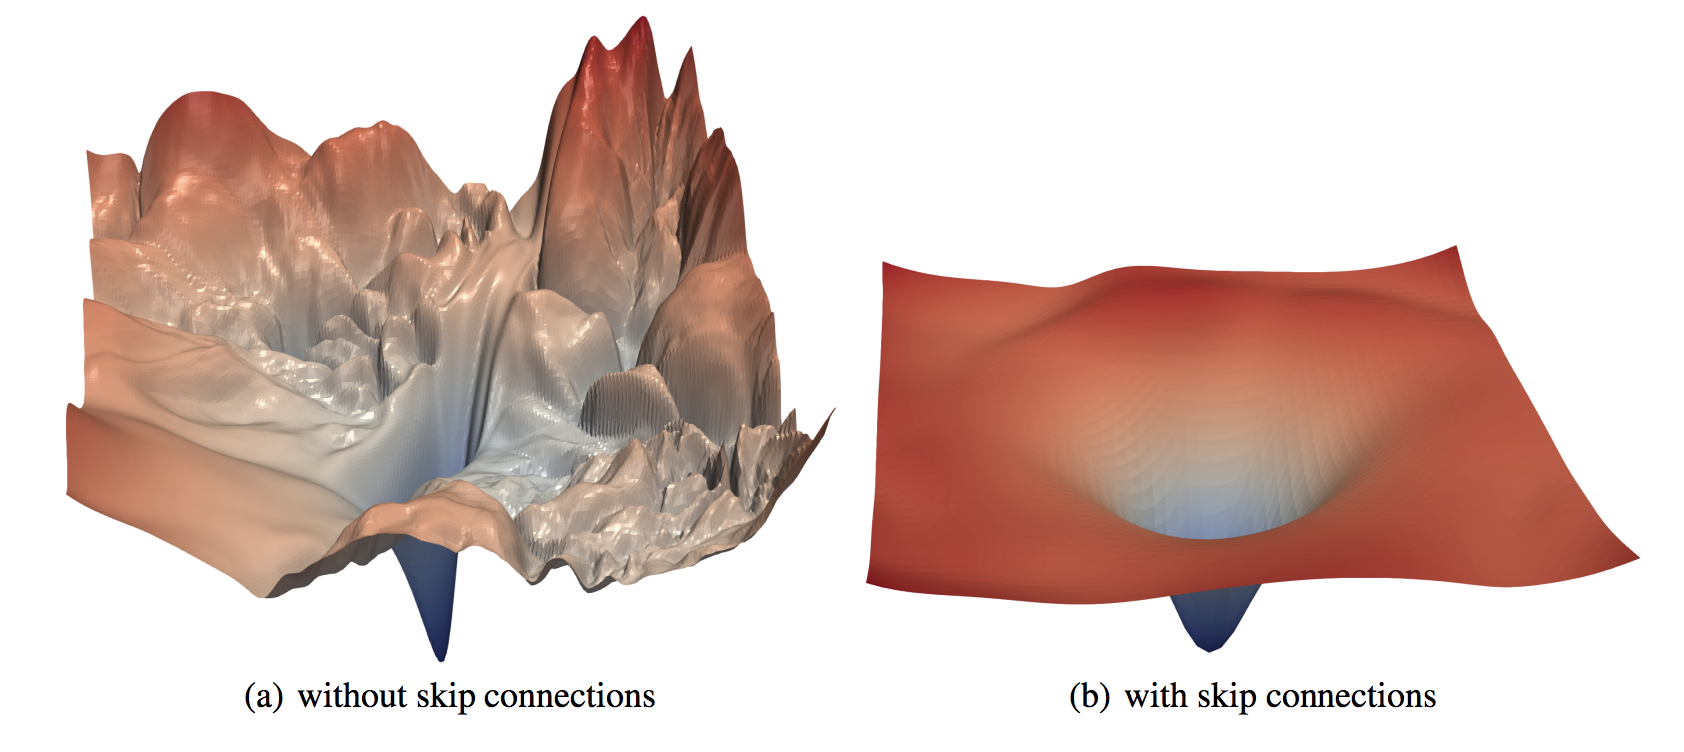
\includegraphics[width=\textwidth]{figs/loss.png}
    \caption{ The loss surfaces of ResNet-56 with/without skip connections.}
    \label{fig:my_label0}
\end{figure}

\section{Information Bottleneck}
% Authors: Joanna Bitton, Divyansh Khanna, Lind Xiao, 2/26/19.
As information moves up the layers, it passes through different layers which filter out relevant features.
This commonly requires altering the dimensions of the information.
For example, recall that one reason pooling is used is to reduce the size of the feature maps.
This dimensionality reduction plays an important role in how the network learns.
The method of extracting relevant information and forgetting the rest is known as a procedure called ``Information Bottleneck".
There has been an increasing interest in the information theory aspect of how deep neural networks work, and how the architectures help them generalize well (\href{https://openreview.net/forum?id=ry_WPG-A-}{paper}).